\PassOptionsToPackage{table}{xcolor}
\documentclass{beamer}

\mode<presentation>
{
  \usetheme{CambridgeUS}      % or try Darmstadt, Madrid, Warsaw, ...
  \usecolortheme{default} % or try albatross, beaver, crane, ...
  \usefonttheme{default}  % or try serif, structurebold, ...
  \setbeamertemplate{navigation symbols}{}
  \setbeamertemplate{caption}[numbered]
} 


\usepackage[spanish]{babel}
\usepackage[utf8x]{inputenc}
\usepackage{algorithm}% http://ctan.org/pkg/algorithms
\usepackage{algpseudocode}% http://ctan.org/pkg/algorithmicx

\title[Análisis y Visualización de Datos MedioAmbientales de Castilla y León]{Análisis y Visualización de Datos MedioAmbientales de Castilla y León}
\subtitle[Diseño y Evaluación de Sistemas Interactivos]{Diseño y Evaluación de Sistemas Interactivos}

\author{Sergio García Prado\\}

\date{17 de Diciembre de 2015}

% Add support for \subsubsectionpage
\def\subsubsectionname{\translate{Subsubsection}}
\def\insertsubsubsectionnumber{\arabic{subsubsection}}
\setbeamertemplate{subsubsection page}
{
  \begin{centering}
    {\usebeamerfont{subsubsection name}\usebeamercolor[fg]{subsubsection name}\subsubsectionname~\insertsubsubsectionnumber}
    \vskip1em\par
    \begin{beamercolorbox}[sep=4pt,center]{part title}
      \usebeamerfont{subsubsection title}\insertsubsubsection\par
    \end{beamercolorbox}
  \end{centering}
}
\def\subsubsectionpage{\usebeamertemplate*{subsubsection page}}

\AtBeginSection{\frame{\sectionpage}}
\AtBeginSubsection{\frame{\subsectionpage}}
\AtBeginSubsubsection{\frame{\subsubsectionpage}}

\begin{document}

%%%%%%%%%%%%%%%

	\begin{frame}
		\titlepage
	\end{frame}

%%%%%%%%%%%%%%%
	
	\begin{frame}
		\tableofcontents
	\end{frame}

%%%%%%%%%%%%%%%

	\section{Introducción}

		\begin{frame}{Objetivos}
 			La representación gráfica de datos medioambientales de la Comunidad Autónoma de Castilla y León. El objetivo de la práctica es descubrir aspectos poco obvios o destacar algo importante del conjunto de datos asignados.

		\end{frame}
		
	\section{Análisis de datos}
	
		\begin{frame}{Adquisición}
			\begin{itemize}
				
				\item El conjunto de datos usado para la práctica contiene información medioambiental de la Comunidad Autónoma de {\bf Castilla y León}.
				
				\item Los datos se pueden encontrar en la web de Datos Abiertos de la Junta de Castilla y León
				\item {\bf Datos Abiertos} es una filosofía y práctica que persigue que determinados tipos de datos estén disponibles de forma libre para todo el mundo, sin restricciones de derechos de autor, de patentes o de otros mecanismos de control. Tiene una ética similar a otros movimientos y comunidades abiertos, como el software libre, el código abierto y el acceso libre.
			\end{itemize}
		
		\end{frame}


		\begin{frame}{Estructura}
		
			\begin{itemize}
			
				\item {\bf Indicador } Campo al que se refiere el dato. Categórico sin Orden.
				
				\item {\bf Provincia } Provincia a la que se refiere el dato. Categórico sin Orden.
				
				\item {\bf Fecha Validez } Fecha en la cual fue obtenido el dato. Cuantitativo.
				
				\item {\bf Valor } Valor que toma el dato respecto de su unidad. Cuantitativo.
				
				\item {\bf Unidad } Unidad de medida del dato. Categórico sin Orden.
				
				\item {\bf Frecuencia } Cantidad de tiempo a la que es referida el dato. Cuantitativo.
			\end{itemize}
		
		\end{frame}
		
		\begin{frame}{Indicadores Escogidos: Producción}
		
			\begin{itemize}
				\item Producción de energía con carbón
				\item Producción de energía eólica
				\item Producción de energía hidráulica
				\item Producción de energía nuclear
				\item Producción de energía primaria
				\item Producción energía solar en Castilla y León	
			\end{itemize}
				
		\end{frame}
		
		\begin{frame}{Indicadores Escogidos: Consumo}
		
			\begin{itemize}
				\item Consumo de energía del sector del transporte
				\item Consumo de energía del sector
				\item Consumo doméstico de electricidad
				\item Consumo doméstico de gas natural
				\item Consumo doméstico de G.L.P.
				\item Consumo doméstico de productos petrolíferos
			\end{itemize}
							
		\end{frame}
		
		\begin{frame}{Transformaciones}
		
			\begin{itemize}

				\item Conversión de todos los datos en {\bf Toneladas Equivalentes de Petróleo} (Tep).
				
				\item {\bf Producción Interna Total}.
				
				\item {\bf Energías Renovables} y {\bf Energías No Renovables}
				
				\item {\bf Consumo Doméstico}.
				
				\item {\bf Producción Externa}.
				
			\end{itemize}

		\end{frame}
		
	\section{Planificación de la Información}

		\begin{frame}{Propósito}
		
			\begin{itemize}
				\item Facilitar la visualización de información al usuario tratando de hacerla lo más clara posible.
			
				\item Sacar conclusiones acerca del flujo energético de Castilla y León. (Explorar los datos)
			
			\end{itemize}
		
		\end{frame}
		
		\begin{frame}{Dualidad}
		
			\begin{itemize}
				\item La información que se va a mostrar corresponde a dos categorías complementarias entre sí (Producción y Consumo).
							
				\item Selección de tonos naranja y azul frente a rojo y verde. (Motivos Socioculturales).
			
			\end{itemize}
		
		\end{frame}

	\section{Diseño}
	
		\subsection{Alternativa 1}
		
			\begin{frame}{Alternativa 1}
				\begin{figure}[H]
					\centering
					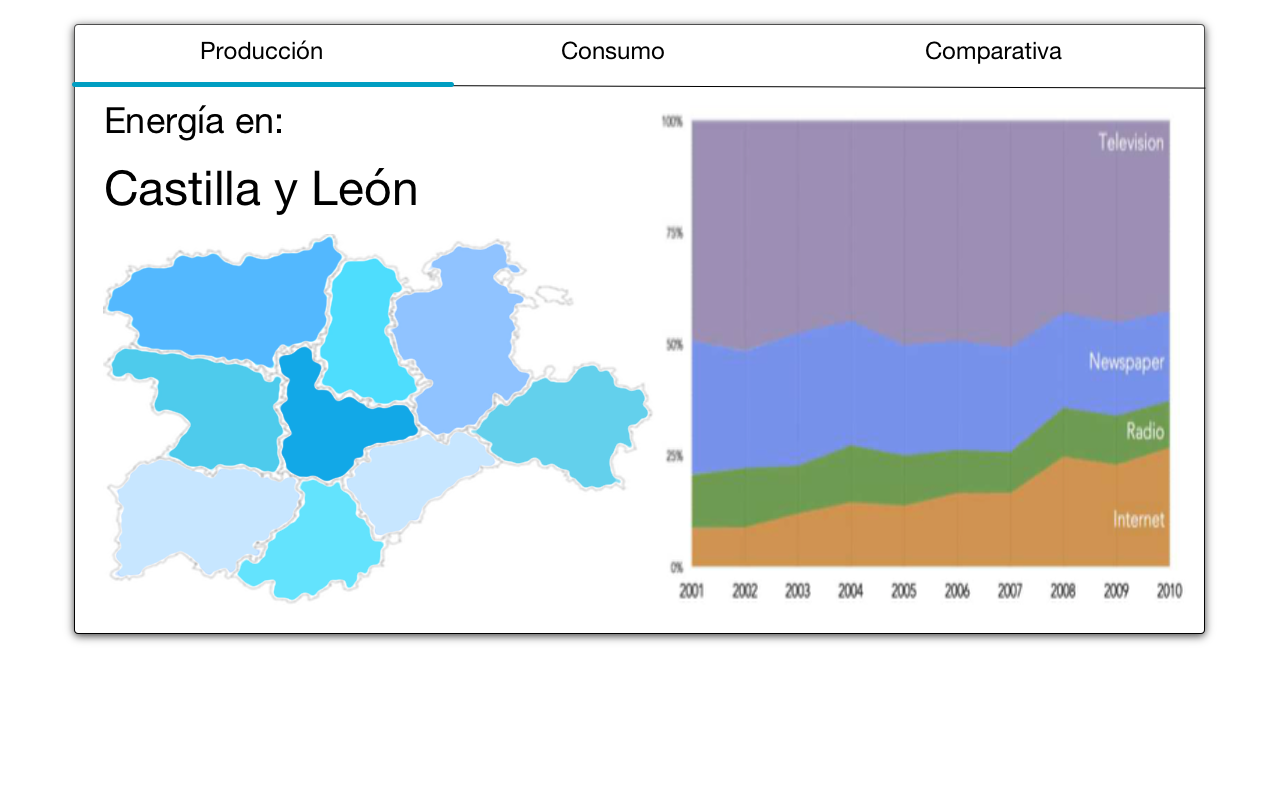
\includegraphics[width=100mm]{../res/design2-1.png}
				\end{figure}
			\end{frame}
			
			\begin{frame}{Alternativa 1}
				\begin{figure}[H]
					\centering
					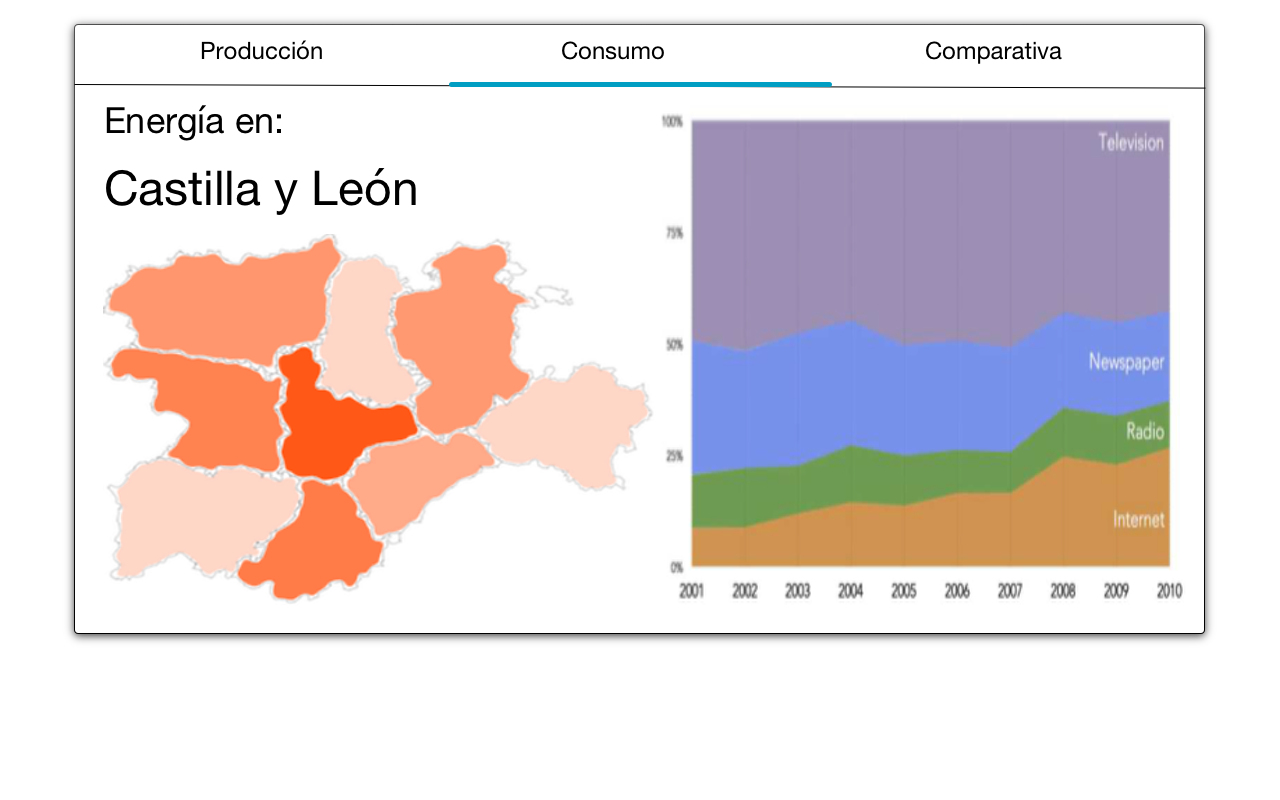
\includegraphics[width=100mm]{../res/design2-2.png}
				\end{figure}
			\end{frame}
			
			\begin{frame}{Alternativa 1}
				\begin{figure}[H]
					\centering
					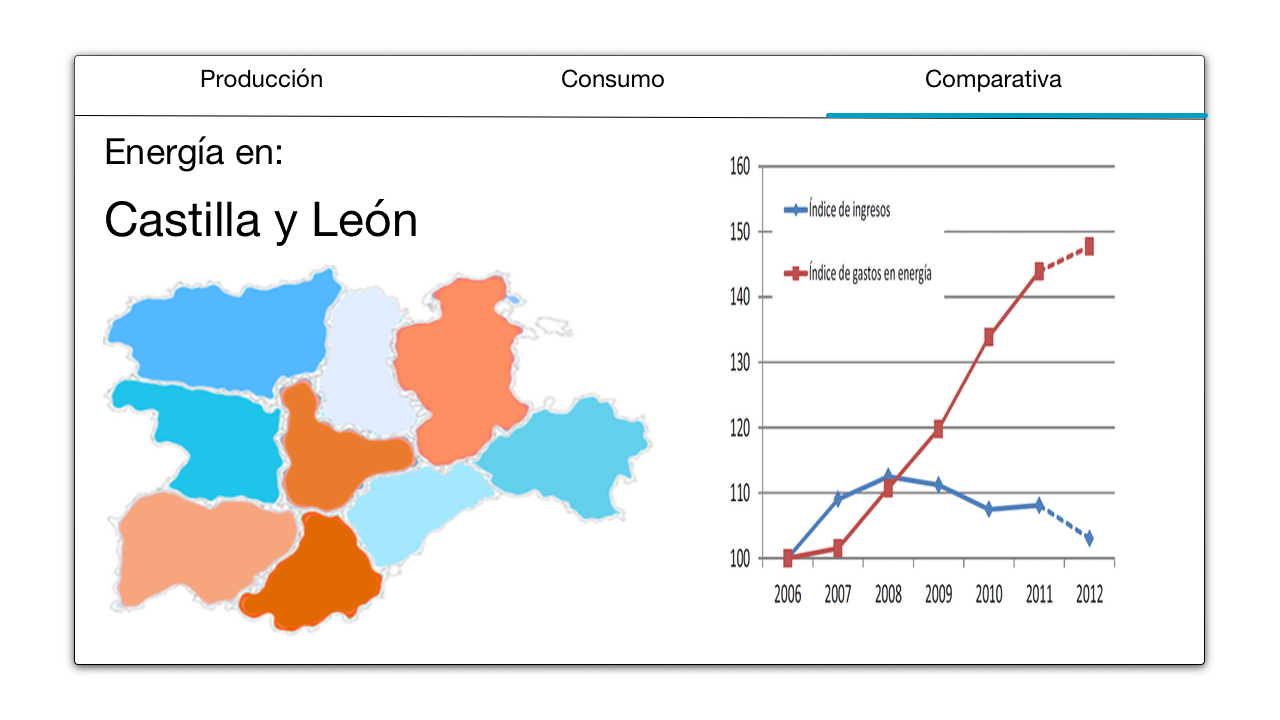
\includegraphics[width=100mm]{../res/design2-3.png}
				\end{figure}
			\end{frame}
		
		\subsection{Alternativa 2}
		
			\begin{frame}{Alternativa 2}
				\begin{figure}[H]
					\centering
					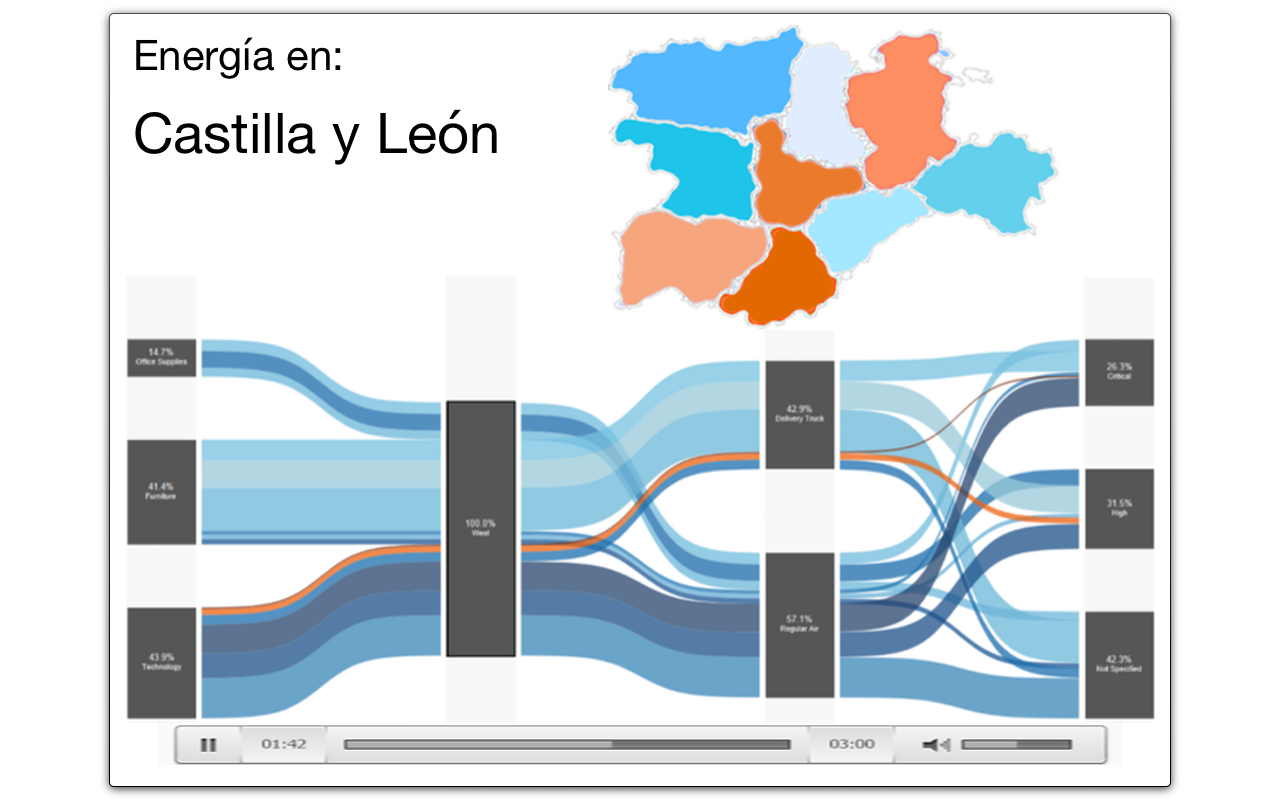
\includegraphics[width=100mm]{../res/design4.png}
				\end{figure}
			\end{frame}
		
		\subsection{Alternativa 3}

			\begin{frame}{Alternativa 3}
				\begin{figure}[H]
					\centering
					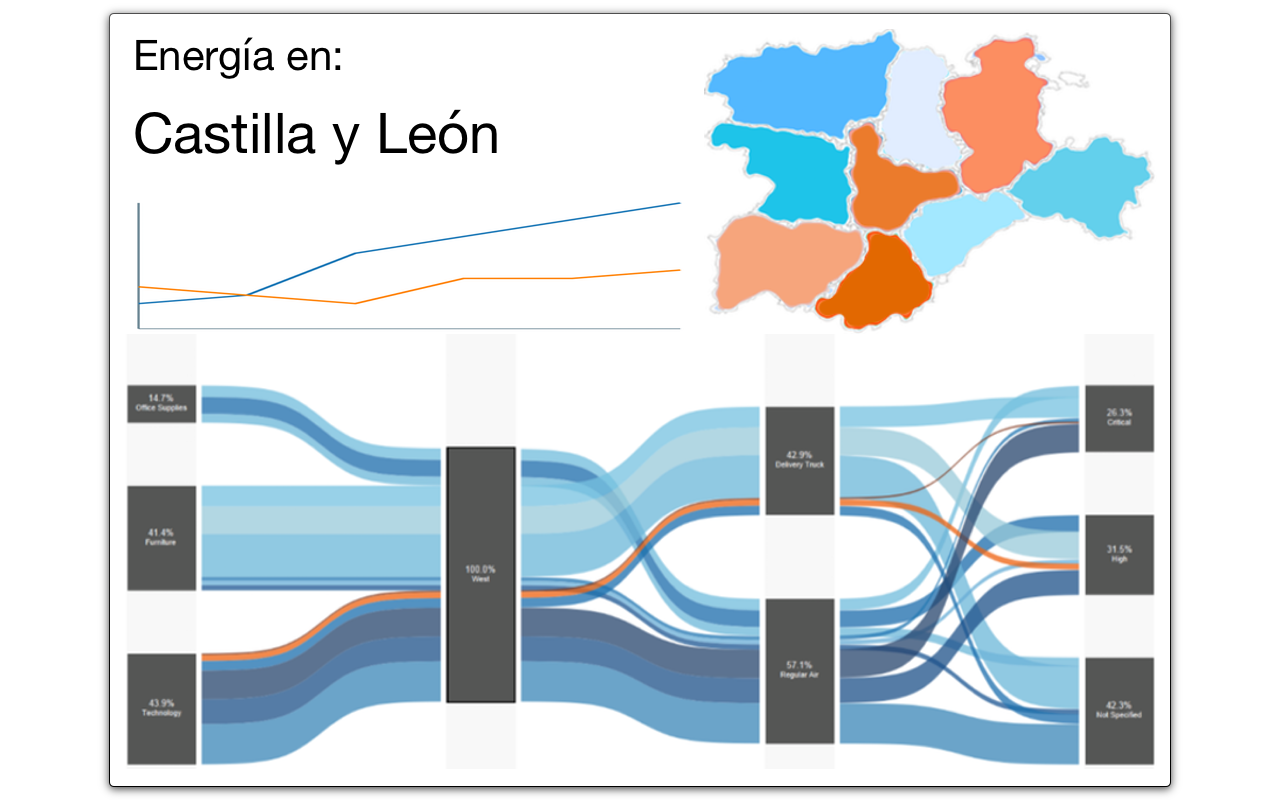
\includegraphics[width=100mm]{../res/design5.png}
				\end{figure}
			\end{frame}
		
	\section{Conclusiones}
	
		\begin{frame}{Conclusiones}
		
			\begin{itemize}
			
				\item Elección de la tercera alternativa porque permite visualizar toda la información en una única vista.
				\item La visualización de datos es algo complicado.
			\end{itemize}
		
		\end{frame}


\end{document}
